\subsection{Towards a Uniform Description Language for Smart Contract}
\label{subsec:uniform-description-language}

Penelitian yang dilakukan oleh \cite{udlsc} mengusulkan sebuah \textit{Uniform Description Language} untuk Smart Contract bernama UDL-SC yang adalah sebuah ekstensi dari USDL. USDL digunakan untuk mendeskripsikan parameter bisnis, operasional, dan teknikal dari \textit{services} yang ada di Internet, sehingga terdapat informasi lainnya seperti \textit{Service Level Agreement} dan hal lainnya. UDL-SC dibangun di atas USDL karena USDL menyediakan deskripsi yang kaya dan komprehensif yang mendeskripsikan parameter \textit{functional} dan \textit{non-functional}. Tujuan dari UDL-SC adalah untuk meningkatkan akses dan pemahaman mengenai Smart Contract dengan sebuah usulan bahasa deskripsi standar.

\begin{figure}[ht]
  \centering
  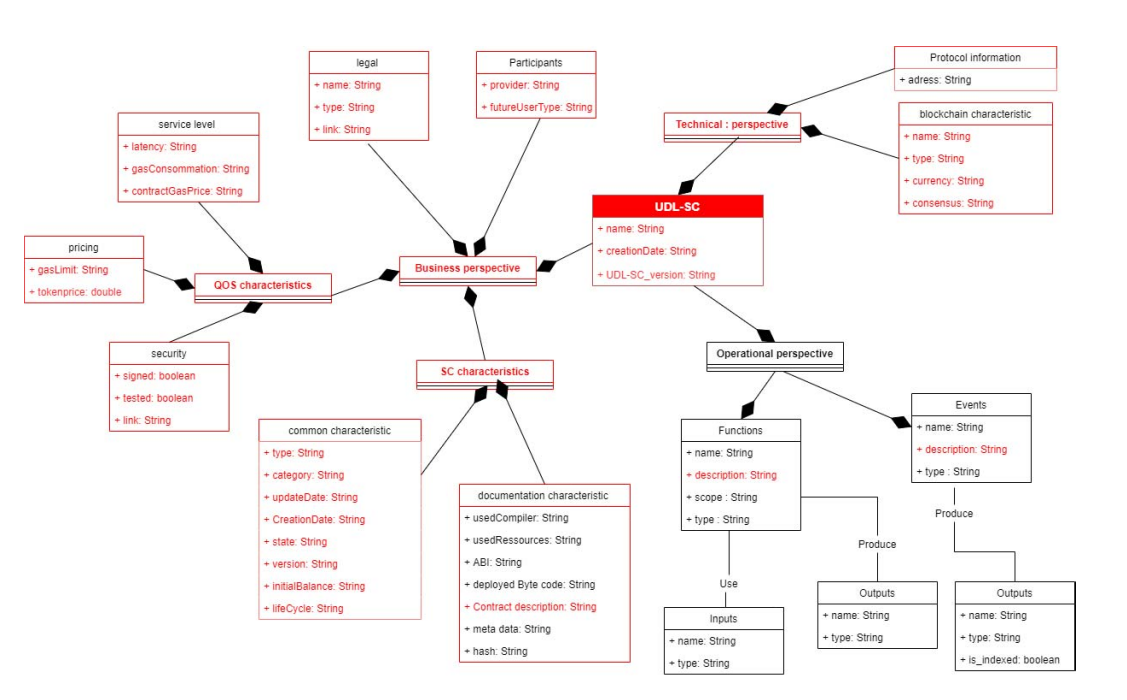
\includegraphics[width=0.7\textwidth]{resources/chapter-2/metamodel-udl-sc.png}
  \caption{Metamodel dari UDL-SC \parencite{udlsc}}
  \label{image:metamodel-udl-sc}
\end{figure}

Metamodel dari UDL-SC dapat dilihat pada Gambar \ref{image:metamodel-udl-sc}. Metamodel dari UDL-SC terdiri dari tiga perspektif utama, yaitu:

\begin{enumerate}
  \item Perspektif Operasional: Berfokus pada atribut fungsional kontrak, seperti fungsi dan event yang dapat dipanggil, beserta parameter yang terlibat.
  \item Perspektif Teknis: Berisi informasi tentang Blockchain tempat kontrak dijalankan, termasuk tipe Blockchain, konsensus, dan protokol yang digunakan.
  \item Perspektif Bisnis: meliputi karakteristik \textit{Quality of Service} (QoS) seperti konsumsi gas, harga gas, serta elemen keamanan dan legal yang terikat pada kontrak, memberikan gambaran yang lebih lengkap dan terperinci mengenai kontrak pintar secara menyeluruh.
\end{enumerate}

\begin{figure}[ht]
  \centering
  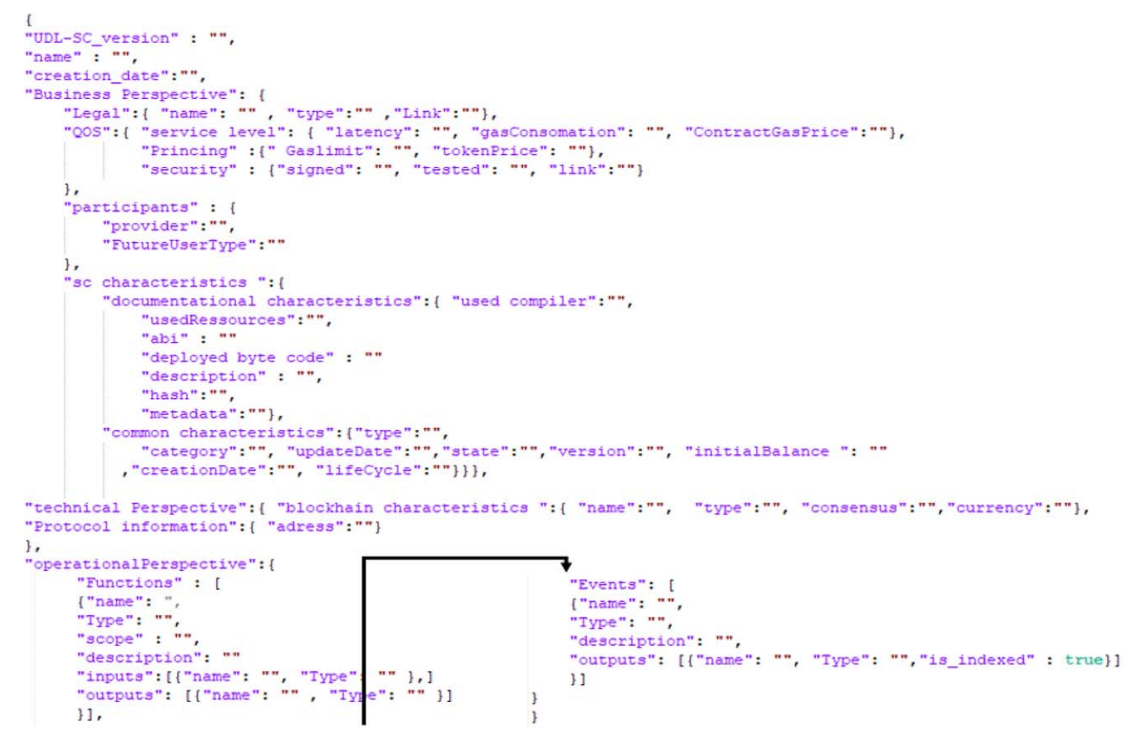
\includegraphics[width=0.7\textwidth]{resources/chapter-2/json-structure-udl-sc.png}
  \caption{Struktur deskripsi umum JSON \parencite{udlsc}}
  \label{image:json-structure-udl-sc}
\end{figure}

Gambar \ref{image:json-structure-udl-sc} menunjukkan deskripsi umum dari struktur UDL-SC dalam format JSON. Dalam penelitian ini, skema JSON dibangkitkan secara otomatis menggunakan kelas Java \texttt{SchemaGenerator}. Proses pembangkitan skema JSON ini dideskripsikan dalam gambar \ref{image:schema-generation-udl-sc}.

\begin{figure}[ht]
  \centering
  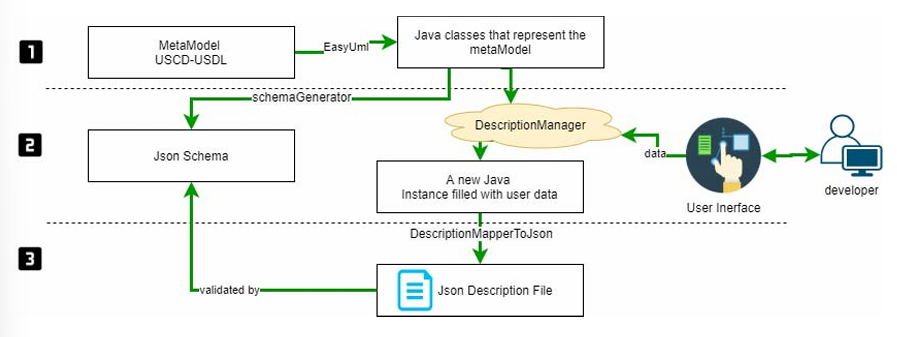
\includegraphics[width=0.7\textwidth]{resources/chapter-2/schema-generation-udl-sc.png}
  \caption{Proses pembangkitan skema JSON \parencite{udlsc}}
  \label{image:schema-generation-udl-sc}
\end{figure}
